\documentclass[12pt,letterpaper]{article}
\usepackage[utf8]{inputenc}
\usepackage[spanish, es-tabla]{babel}
\usepackage[version=3]{mhchem}
\usepackage[journal=jacs]{chemstyle}
\usepackage{amsmath}
\usepackage{amsfonts}
\usepackage{amssymb}
\usepackage{makeidx}
\usepackage{xcolor}
\usepackage[stable]{footmisc}
\usepackage[section]{placeins}
%Paquetes necesarios para tablas
\usepackage{longtable}
\usepackage{array}
\usepackage{xtab}
\usepackage{multirow}
\usepackage{colortab}
\usepackage{caption}
\usepackage{enumitem}
%Paquete para el manejo de las unidades
\usepackage{siunitx}
\sisetup{mode=text, output-decimal-marker = {,}, per-mode = symbol, qualifier-mode = phrase, qualifier-phrase = { de }, list-units = brackets, range-units = brackets, range-phrase = --}
\usepackage{cancel}
%Paquetes necesarios para imágenes, pies de página, etc.

%Instrucción para evitar la indentación
%\setlength\parindent{0pt}
%Paquete para incluir la bibliografía
\usepackage[backend=bibtex,style=chem-acs,biblabel=dot]{biblatex}
\addbibresource{references.bib}


%Modificación del formato de los captions
\usepackage[margin=10pt,labelfont=bf]{caption}

%Paquete para incluir comentarios
\usepackage{todonotes}

%Paquete para incluir hipervínculos
\usepackage[colorlinks=true, 
            linkcolor = blue,
            urlcolor  = blue,
            citecolor = black,
            anchorcolor = blue]{hyperref}
            
            

\begin{document}
\renewcommand{\labelitemi}{$\checkmark$}

\renewcommand{\CancelColor}{\color{red}}

\newcolumntype{L}[1]{>{\raggedright\let\newline\\\arraybackslash}m{#1}}

\newcolumntype{C}[1]{>{\centering\let\newline\\\arraybackslash}m{#1}}

\newcolumntype{R}[1]{>{\raggedleft\let\newline\\\arraybackslash}m{#1}}

\begin{center}
	\textbf{\LARGE{TUTORIAL 1 DE NETLOGO}}\\
	\vspace{7mm}
	\textbf{\large{Realizado Por: Michael Santiago Díaz 160002613}}\\
	\textbf{\large{Entregado A: Ph.D Ángel Cruz}}\\
	\vspace{5mm}
	\textbf{\large{Universidad de los llanos}}\\
	\today
\end{center}

\vspace{10mm}
\begin{itemize}
	\renewcommand{\labelitemi}{\scriptsize$\blacksquare$} 
	
	
	
	\item Abra Models Library del menú File
	
	\item Elija "Wolf Sheep Predation" de la sección Biology y pulse "Open"
	
	\item Presione el botón "setup"
		\paragraph{Pregunta:}	
			¿Qué le aparece en la vista?
	
		\subparagraph{respuesta:}
			Aparece una simulación completa lista para ser ejecutada, con los controladores ya sean botones y sliders, una vista para visualizar la el resultado de la simulación y una gráfica que muestra el valor de las variables a estudiar con respecto al tiempo, que este contexto se llaman ticks.
			
			\begin{center}
				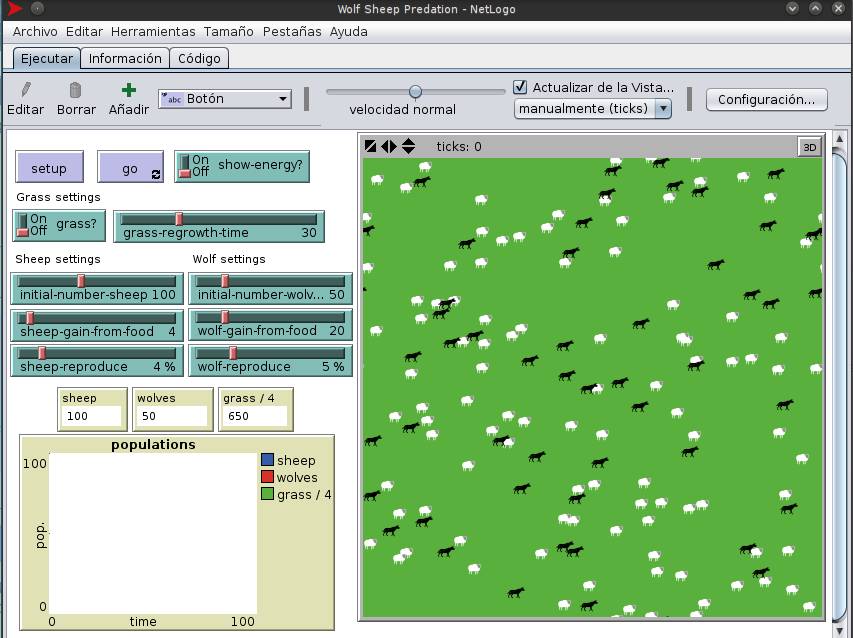
\includegraphics[width=8cm]{./imagenes/image1.png}
			\end{center}
%------------------------------------------

%------------------------------------------

	\item Presione el botón "go" para iniciar la simulación.
	\item Presione el botón "go" para detener el modelo.
		\paragraph{Pregunta:}
			¿Qué le está sucediendo a las poblaciones de lobos y ovejas a medida que está corriendo el modelo?
			
		\subparagraph{respuesta:}
			En la simulación se dio el caso de que a medida que la población de ovejas crecía, la población de lobo también lo hacía pero llega un momento en que la población de ovejas no es capaz de mantener a la población de lobos y estos mueren, se da el caso que algunas ovejas sobreviven y luego se reproducen infinitamente.
			\begin{center}
				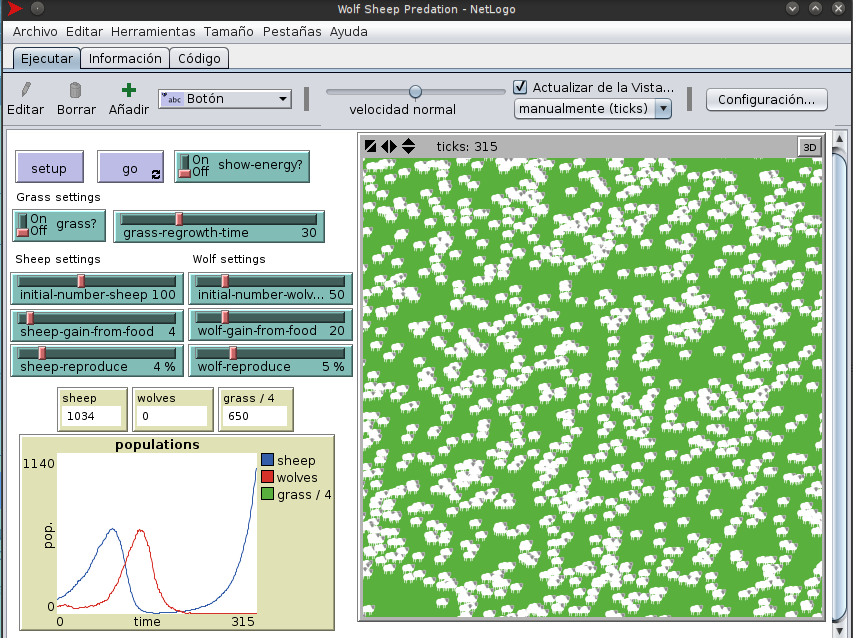
\includegraphics[width=8cm]{./imagenes/image2.png}
			\end{center}

	\paragraph{Pregunta:}
	¿Alguna vez obtendrá resultados diferentes si ejecuta el modelo en repetidas ocasiones manteniendo la misma configuración?
	
	\begin{figure}
	\centering
		\begin{minipage}{.5\textwidth}
			\centering
			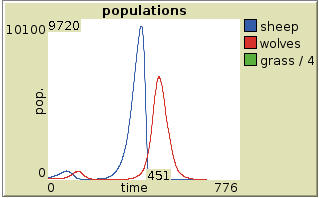
\includegraphics[width=7cm]{./imagenes/image3.png}
		\end{minipage}%
		\begin{minipage}{.5\textwidth}
  			\centering
  			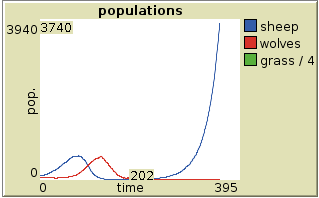
\includegraphics[width=7cm]{./imagenes/image4.png}
		\end{minipage}
	\end{figure}

	\subparagraph{respuesta:}
		Así es suceden dos casos distinto:
		\begin{itemize}
			\item la población de lobos crece demasiado y extermina la población de ovejas y luego la población de lobos muere por falta de alimento.
		
			\item la población de lobos aumenta y cerca de la extinción de las ovejas unas pocas se salvan, los lobos mueren por falta de alimento y la población de ovejas que cuenta con pasto ilimitadamente crece infinitamente.
		\end{itemize}
	
	\hfill \\
		
	\item Abra Wolf Sheep Predation si aún no está abierto.
	
	\item Presione 'setup' y 'go' y deje que el modelo corra por aproximadamente 100 ticks de tiempo. (Nota: hay una lectura del número de ticks justo encima de la parcela).
	
	\item Detenga el modelo pulsando el botón "go".

		\paragraph{pregunta:}
			¿Qué pasó con las ovejas a través del tiempo?
			
		\subparagraph{respuesta:}
			Las ovejas tienden a la extinción
			
			\begin{center}
				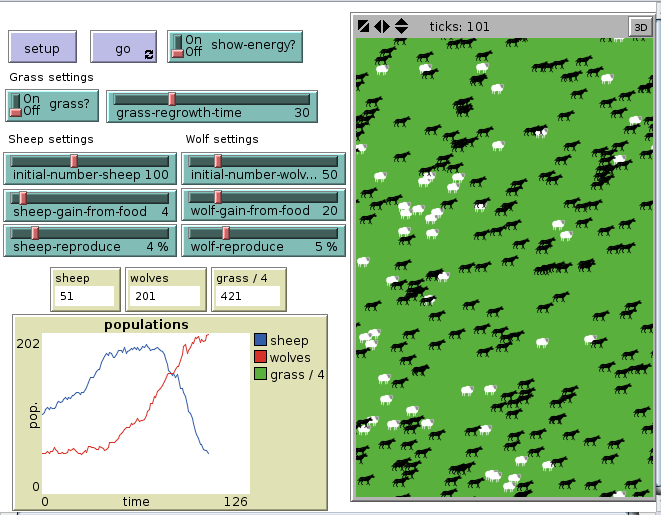
\includegraphics[width=8cm]{./imagenes/image5.png}
			\end{center}
			
		
	Echemos un vistazo y veamos que les sucedería a las ovejas si cambiásemos alguno de los ajustes en la configuración.
	\hfill \
	
	\item Encienda el switch de  la hierba ("grass?").
	\item Presione "setup" y "go" y deje correr el modelo por una cantidad de tiempo similar al de la anterior.
	
		\paragraph{pregunta: }
			¿Qué le hizo este switch al modelo? ¿Fue el mismo resultado de la ejecución previa?

		\subparagraph{respuesta:}		
			la población de ovejas es más grande en el mismo instante de tiempo, puede ser debido a q con la falta de comida en ciertas áreas las ovejas se mueven y a los lobos les es más difícil comerlas, haciendo que su población disminuya.

			\begin{center}
				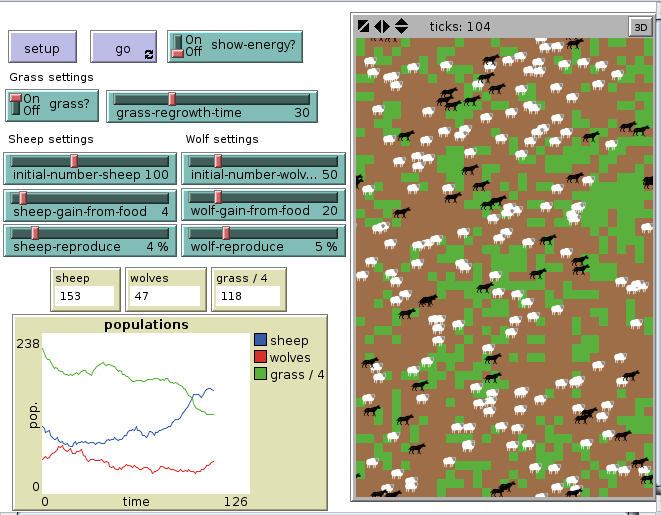
\includegraphics[width=8cm]{./imagenes/image6.png}
			\end{center}
	
	Vamos a investigar los sliders de la depredación lobo oveja.
	\item Lea el contenido de la ficha de Información, localizado arriba en la barra de herramientas, para aprender lo que representa cada uno de los sliders de este modelo
	
		\begin{itemize}	
			\item INITIAL-NUMBER-SHEEP: The initial size of sheep population
			\item INITIAL-NUMBER-WOLVES: The initial size of wolf population
			\item SHEEP-GAIN-FROM-FOOD: The amount of energy sheep get for every grass patch eaten
			\item WOLF-GAIN-FROM-FOOD: The amount of energy wolves get for every sheep eaten
			\item SHEEP-REPRODUCE: The probability of a sheep reproducing at each time step
			\item WOLF-REPRODUCE: The probability of a wolf reproducing at each time step
			\item GRASS?: Whether or not to include grass in the model
			\item GRASS-REGROWTH-TIME: How long it takes for grass to regrow once it is eaten
			\item SHOW-ENERGY?: Whether or not to show the energy of each animal as a number
		\end{itemize}
		
	\paragraph{pregunta:}
		¿Qué sucedería con la población de ovejas si hay al comienzo de la simulación inician más ovejas y menos lobos?
		
		\begin{itemize}
			\item Apague "grass".
			\item Establezca el slider del número inicial de ovejas ( "initial-number-sheep") a 100.
			\item Establezca el slider del número inicial de lobos ("initial-number-wolves") a 20.
			\item Presione "setup" y luego "go".
			\item Permita que el modelo corra alrededor de 100 ticks de tiempo.

		\end{itemize}
		
		\begin{center}
				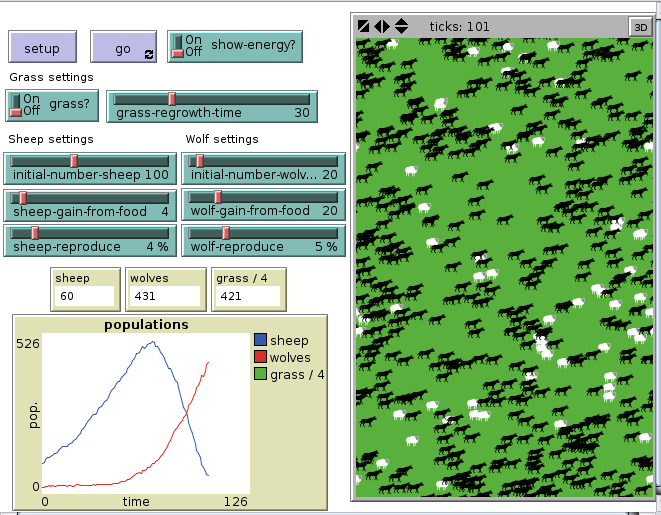
\includegraphics[width=8cm]{./imagenes/image7.png}
		\end{center}
		
	Intente correr el modelo varias veces con estos ajustes.
	
	\paragraph{pregunta:}
		¿Qué le ocurrió a la población de ovejas?
		
	\subparagraph{respuesta}
		las repetidas simulaciones con los mismos parámetros conllevan  mismo resultado en las 100 repeticiones (población de ovejas disminuyendo) el único cambio es que las poblaciones de lobos y ovejas llegan a picos más altos antes de la caída de la población de ovejas
		
	\begin{figure}
	\centering
		\begin{minipage}{.5\textwidth}
			\centering
			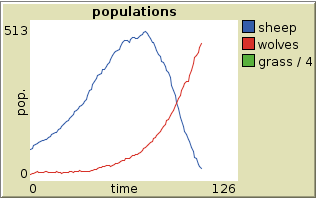
\includegraphics[width=7cm]{./imagenes/image8.png}
		\end{minipage}%
		\begin{minipage}{.5\textwidth}
  			\centering
  			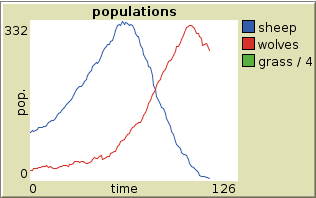
\includegraphics[width=7cm]{./imagenes/image9.png}
		\end{minipage}
	\end{figure}
	\begin{figure}
	\centering
		\begin{minipage}{.5\textwidth}
			\centering
			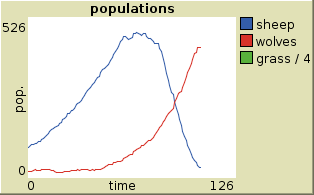
\includegraphics[width=7cm]{./imagenes/image10.png}
		\end{minipage}%
		\begin{minipage}{.5\textwidth}
  			\centering
  			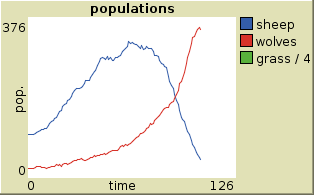
\includegraphics[width=7cm]{./imagenes/image11.png}
		\end{minipage}
	\end{figure}
	
	\paragraph{pregunta:}
		¿Le sorprendió este resultado?, ¿Qué otros sliders o switches se pueden ajustar para ayudarle a la población de ovejas?
		
	\subparagraph{respuesta:}
		se puede aumentar la tasa de reproducción de las ovejas esto hará que su número crezca exponencialmente y superen por mucho a los lobos
		\begin{center}
			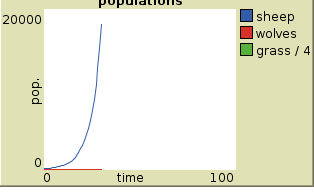
\includegraphics[width=7cm]{./imagenes/image12.png}
		\end{center}
		
		disminuir la tasa de reproducción de los lobos
		
		\begin{center}
			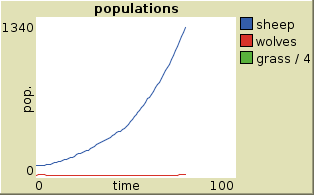
\includegraphics[width=7cm]{./imagenes/image13.png}
		\end{center}
		
		los otros slider por separados solo retrasan el resultado mas comun que es que la poblacion de lobos debora completamente la poblacion de ovejas
		
		\hfill \\
		
	Ajuste el número inicial de ovejas a 80  y el número inicial de lobos a 50. (Esto es cercano a la forma en que estaban cuando usted abrió el modelo por primera vez.)
	
	\item Fije "sheep-reproduce" en 10,0%.
	\item Presione "setup" y luego "go".
	\item Permita que el modelo corra alrededor de 100 ticks de tiempo.
	
	\paragraph{pregunta:}	
		¿Qué le pasó a los lobos en esta ejecución?
	
		\subparagraph{respuesta:}
			como puede observarse la población de lobos y ovejas se disparó, las ovejas al reproducirse más y los lobos al poseer una mayor fuente de alimento no morían ya que su energía nunca disminuía.
			
			\begin{center}
				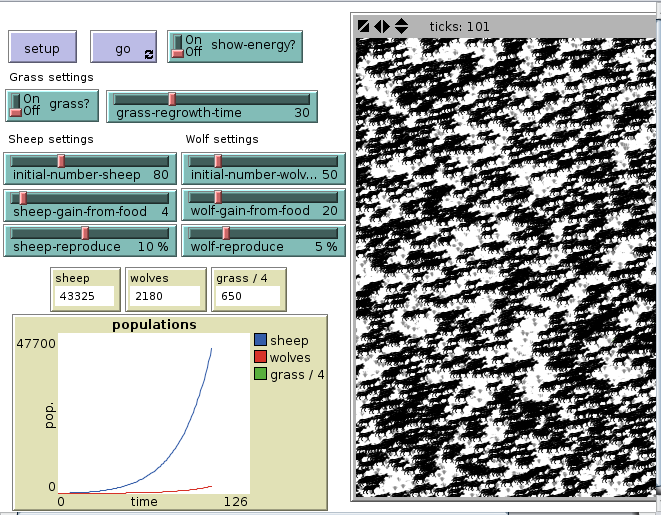
\includegraphics[width=7cm]{./imagenes/image14.png}
			\end{center}
	
	\hfill \\
	\hfill \\	
	
	\begin{center}
		CONTROL DE LA VISTA
	\end{center}
	
	Vamos a experimentar con el efecto de estos controles.
 	
 	\item Presione "setup" y luego "go" para iniciar la ejecución del modelo.

	\item A medida que corra el modelo, mueva el slider de la velocidad a la izquierda.

	\paragraph{pregunta:}
		¿Qué sucede?
		\subparagraph{respuesta:}
			La ejecución se realiza más lentamente a medida que la barra se acerca al extremo izquierdo

	Este slider es útil si un modelo se está ejecutando demasiado rápido como para que usted pueda ver en detalle lo que está pasando.
	
	\item Mueva el slider de velocidad a la mitad.

	\item Pruebe moviendo el slider de la velocidad a la derecha.

	\item Ahora intente marcando y desmarcando la casilla de verificación de las actualizaciones de la vista (view updates).

	\paragraph{pregunta:}
		¿Qué sucede?

		\subparagraph{respuesta:} al momento de checkear nuevamente la visualización la vista se actualiza, al quitar el check la visualización se detiene pero la simulación sigue ejecutándose


	Pulse el botón "Settings ..." en la barra de herramientas.

	\item Se abrirá un cuadro de diálogo que contiene todos los ajustes para la vista:
	
	\paragraph{pregunta:}
		¿Cuáles son los ajustes actuales para max-pxcor, pxcor-min, max-pycor, min-pycor, y patch size (tamaño del parche)?
	
	\subparagraph{repuesta:}	
		Minpxcor: -25, maxpxcor: 25, minpycor: -25, maxpycor: 25, pathsize: 9

	La vista está seleccionada ahora, cosa que usted puede saber porque la vista ahora está rodeada por un borde gris.

	\item Arrastre una de las "asas" cuadradas negras. Las asas se encuentran en los bordes y en las esquinas de la vista.
	
	\item Deseleccione la vista haciendo clic en cualquier lugar del fondo blanco de la Interfaz.
	
	\item Pulse de nuevo el botón "Settings..." y vea los ajustes.
	
	\paragraph{pregunta:}
		¿Qué números cambiaron?
		
	\subparagraph{respuesta:}		
		Path size: 5.7
		
	\paragraph{pregunta:}
		¿Qué números no cambiaron?
		
	\subparagraph{respuesta:}		
		Solo path size fue modificado
		
	\paragraph{pregunta:}
		¿A cuántas baldosas de distancia está la baldosa (0,0) respecto a lado derecha de la habitación?
		
	\subparagraph{respuesta:}		
		25
		
	\paragraph{pregunta:}
		¿A Cuántas baldosas de distancia está la baldosa (0,0) respecto al lado izquierdo de la habitación?
		
	\subparagraph{respuesta:}		
		25


	\item Utilizando el diálogo de Model Settings que aun sigue abierto, cambie max-pxcor a 30 y el valor de max-pycor a 10. Observe que min-pxcor min-pycor también cambian. 
	
	\hfill \\	
	
	Esto se debe a que por defecto el origen (0,0) está en el centro del mundo.
	
	
	\paragraph{pregunta:}
		¿Qué le ocurrió a la forma de la vista?

	\subparagraph{respuesta:}		
		se volvió de forma rectangular

	\item Presione el botón de "setup".
	
	\item Ahora puede ver los nuevos parches que ha creado.

	\item Edite la vista pulsando nuevamente el botón "Settings...".

	\item Cambie el tamaño del parche (patch size) a 20 y presione "OK".

	\paragraph{pregunta:}		
		¿Qué pasó con el tamaño de la vista?, ¿cambió esto su forma?
	
	\subparagraph{respuesta:}
		el tamaño de la vista aumento pero la cantidad de cuadros es la misma

	
\end{itemize}
%------------------------------------------


\end{document}
